\documentclass[a4paper,12pt]{article}
\usepackage[utf8]{inputenc}
\usepackage{amsmath}
\usepackage{amsfonts}
\usepackage{amssymb}
\usepackage{graphicx}
\usepackage{hyperref}
\usepackage{geometry}
\usepackage{fancyhdr}

\pagestyle{fancy}
\fancyhf{}
\renewcommand{\headrulewidth}{0.4pt} % full-width rule
\fancyhead[L]{EEE F313: ADVD Lab 1 Report}
\fancyhead[R]{Pramit Pal}
\fancyfoot[C]{\thepage}

\geometry{a4paper, margin=1in}
\title{EEE F313: ADVD Lab 1 Report}
\author{Pramit Pal \\ 2023AAPS0765}
\date{}

\begin{document}
\maketitle
\section{Introduction}
The first lab involved learning how to access and user virtuoso, as well as create and use a basic circuit. We were required to then plot $I_D$ against $V_{DS} \& V_{GS}$ as well as $V_{GS}$ against $V_{DS}$ for an NMOS and PMOS transistor in a basic circut.

We were also required to identify $V_{th}$ from the graphs.

\section{NMOS Characteristics}
The NMOS circuit is shown in figure \ref{fig:nmos_circuit}.
\begin{figure}[h!]
	\centering
	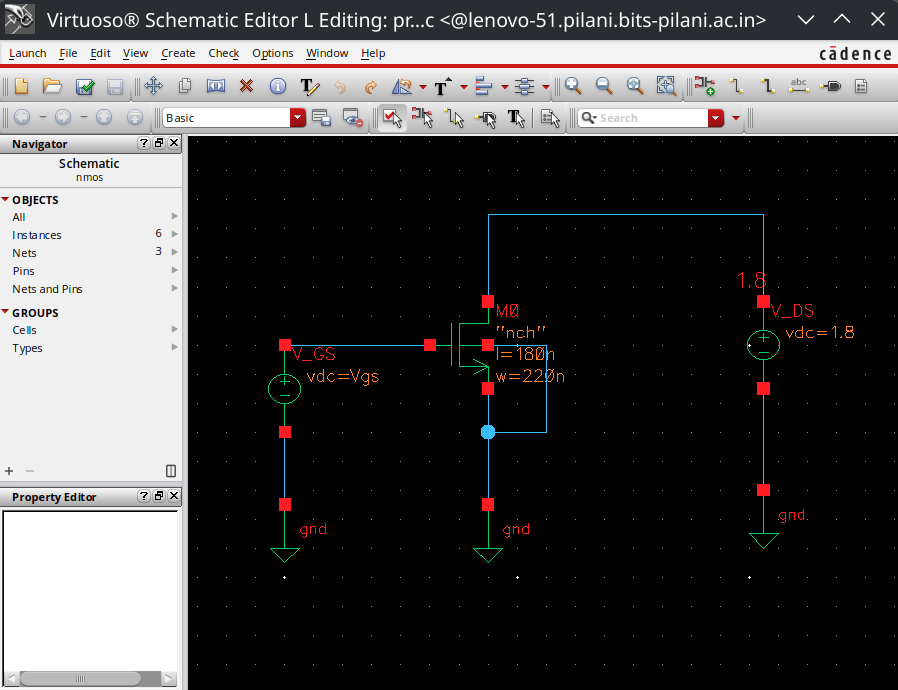
\includegraphics[width=0.8\textwidth]{images/nmos-circuit.png}
	\caption{NMOS Circuit}
	\label{fig:nmos_circuit}
\end{figure}

The values for $V_{DS}$ were varied between 0V and 1.8V, with a step size of 0.01V. A DC analysis was plotted, with the NMOS parameters being $l = 180nm$, $w = 220nm$, and $V_{GS} = 1.8V$.

\subsection{NMOS Characteristics}
Upon performing the plot, the following graph was obtained:
\begin{figure}[h!]
	\centering
	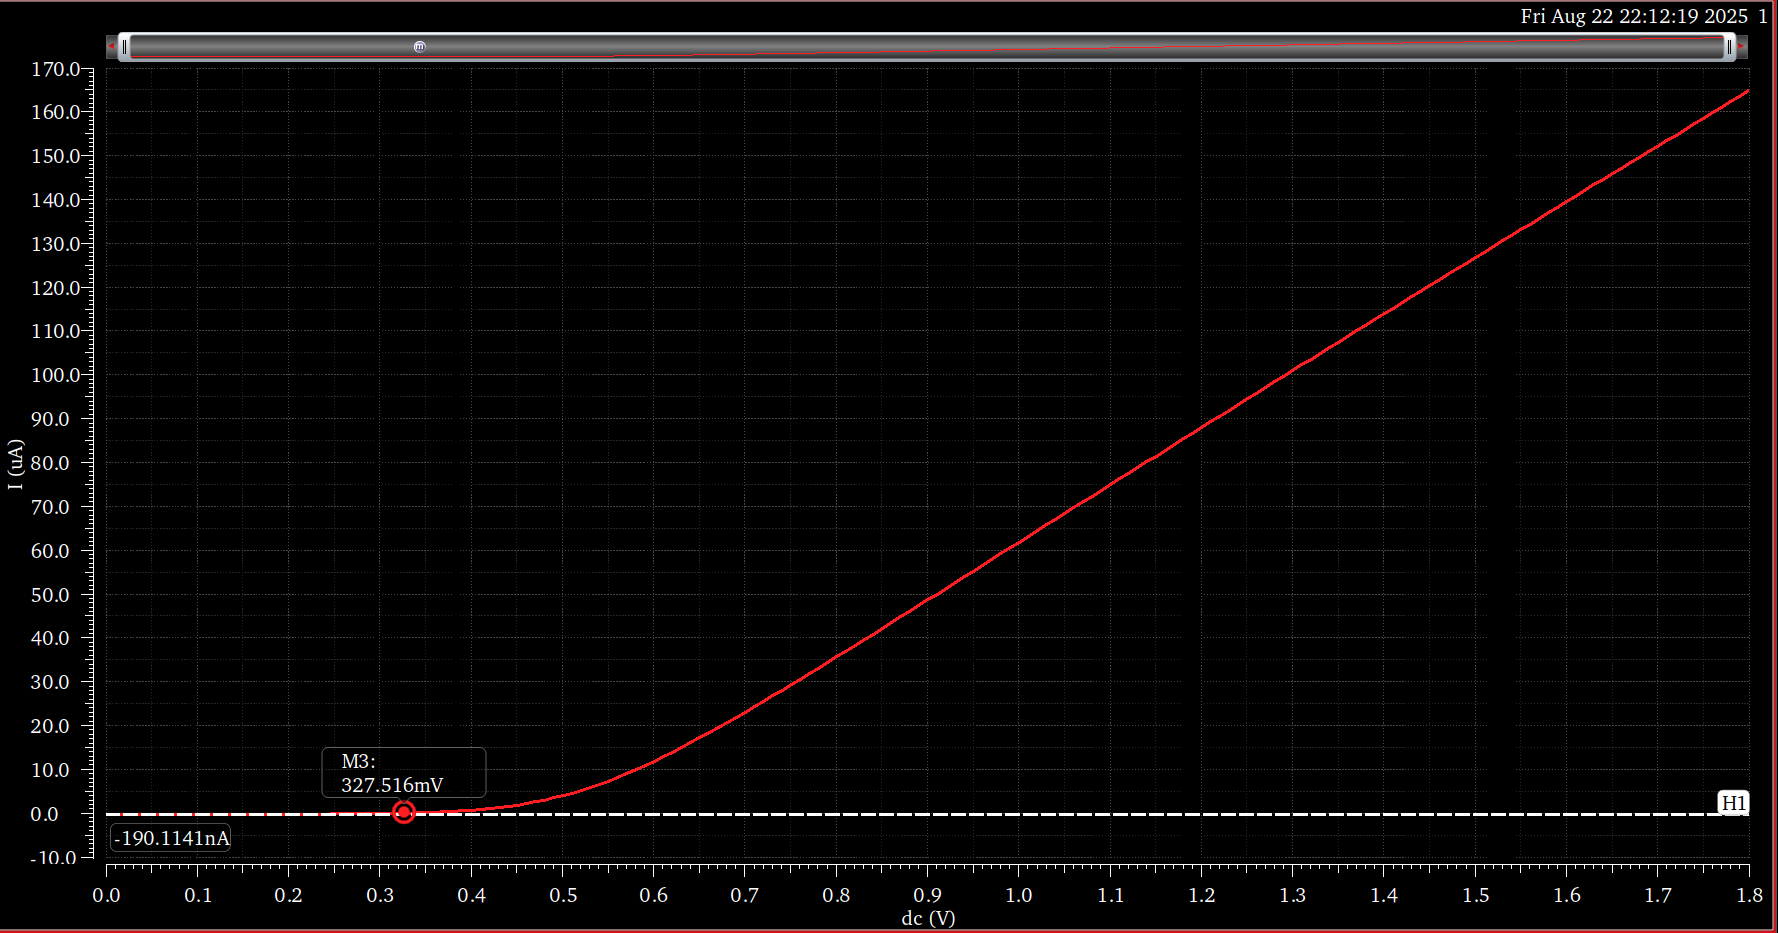
\includegraphics[width=0.8\textwidth]{images/nmos-I_D-vs-V_GS.png}
	\caption{$I_D$ vs $V_{GS}$ for NMOS}
	\label{fig:nmos-id-vs-vgs}
\end{figure}
From \ref{fig:nmos-id-vs-vgs}, we can see that the threshold voltage $V_{th}$ is approximately 0.4V, as this is where the current $I_D$ starts to increase significantly.
\subsection{$I_D$ vs $V_{DS}$ for NMOS}
The following graph was obtained for $I_D$ vs $V_{DS}$:
\begin{figure}[h!]
	\centering
	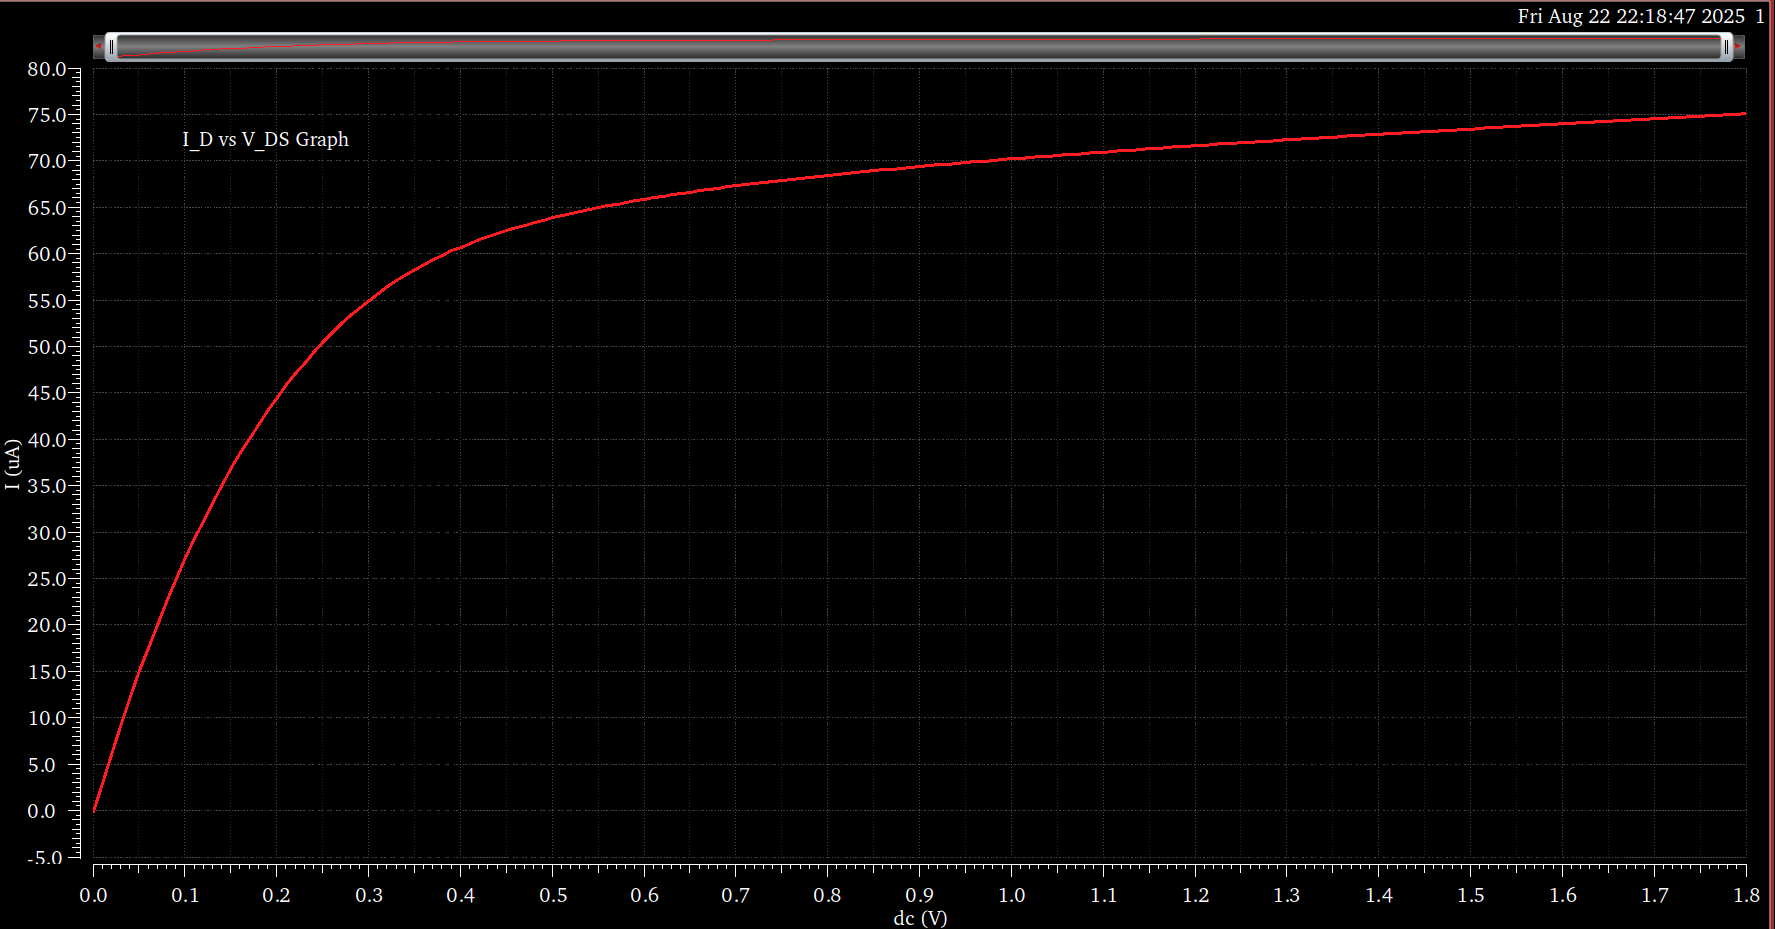
\includegraphics[width=0.8\textwidth]{images/nmos-I_D-vs-V_DS.png}
	\caption{$I_D$ vs $V_{DS}$ for NMOS}
	\label{fig:nmos-id-vs-vds}
\end{figure}

\newpage
\subsection{$I_D$ against $V_{DS} \& V_{GS}$ for NMOS}
As an extension, various values of $V_{GS}$ were used to plot $I_D$ against $V_{DS}$, resulting in the graph shown in figure \ref{fig:nmos-id-vs-vds-vgs}.
\begin{figure}[h!]
	\centering
	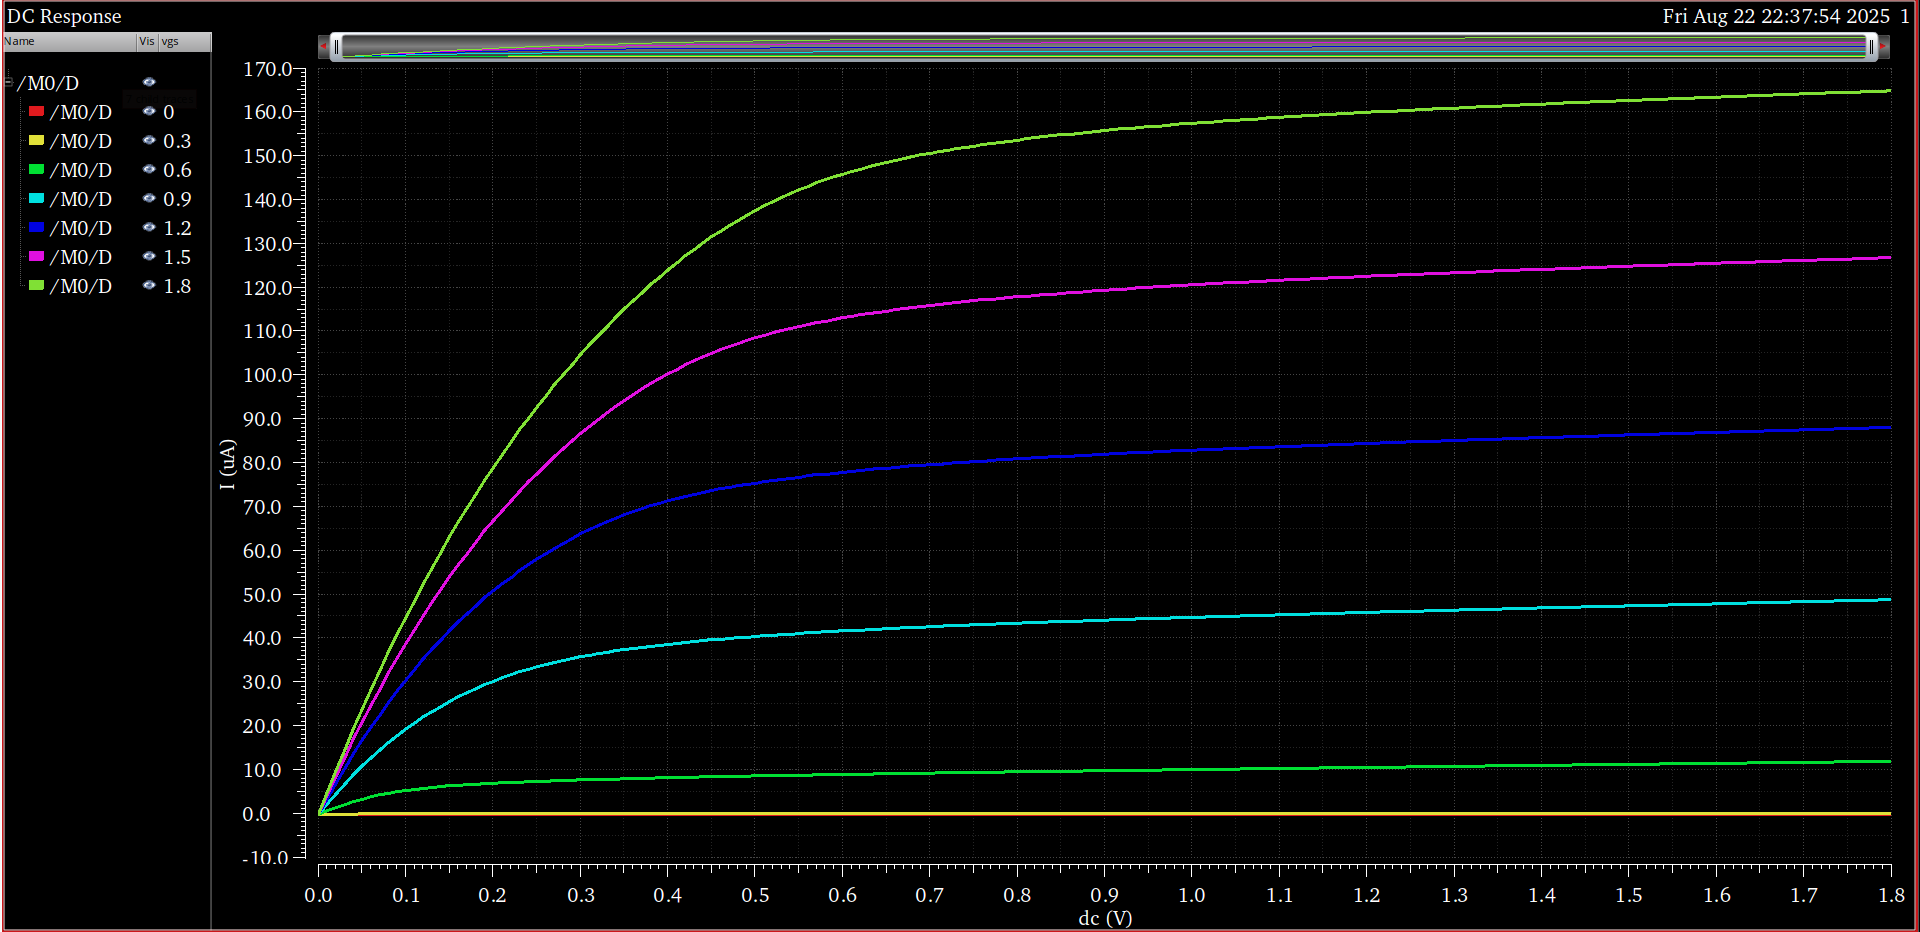
\includegraphics[width=0.8\textwidth]{images/nmos-I_D-vs-V_DS-at-V_GS.png}
	\caption{$I_D$ vs $V_{DS}$ for various $V_{GS}$ values}
	\label{fig:nmos-id-vs-vds-vgs}
\end{figure}

You can see how the value of $V_{GS}$ affects the $I_D$ vs $V_{DS}$ curve, with higher $V_{GS}$ values leading to higher $I_D$ values for the same $V_{DS}$. Additionally, you can see how the triode region shifts right as the value of $V_{GS}$ increases.

\newpage
\section{PMOS Characteristics}
The PMOS circuit was set up similarly to the NMOS circuit, with the PMOS parameters being $l = 180nm$, $w = 220nm$, and $V_{SG} = 1.8V$. The circuit is shown in figure \ref{fig:pmos_circuit}.
\begin{figure}[h!]
	\centering
	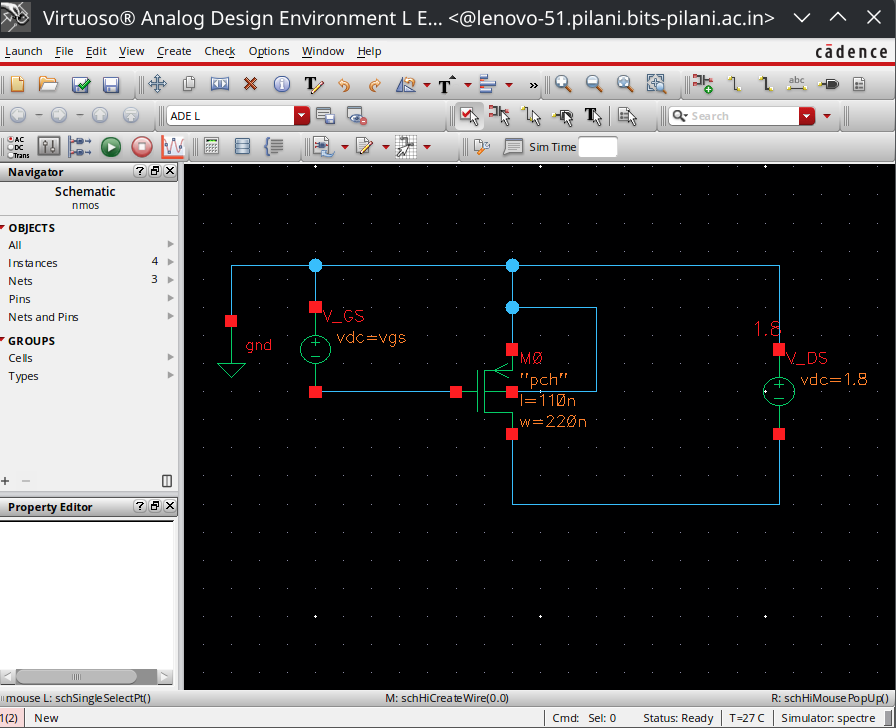
\includegraphics[width=0.8\textwidth]{images/pmos-circuit.png}
	\caption{PMOS Circuit}
	\label{fig:pmos_circuit}
\end{figure}

\subsection{$I_D$ vs $V_{DS}$ for PMOS}
The following graph was obtained for $I_D$ vs $V_{DS}$ for the PMOS circuit from figure \ref{fig:pmos_circuit}:
\begin{figure}[h!]
	\centering
	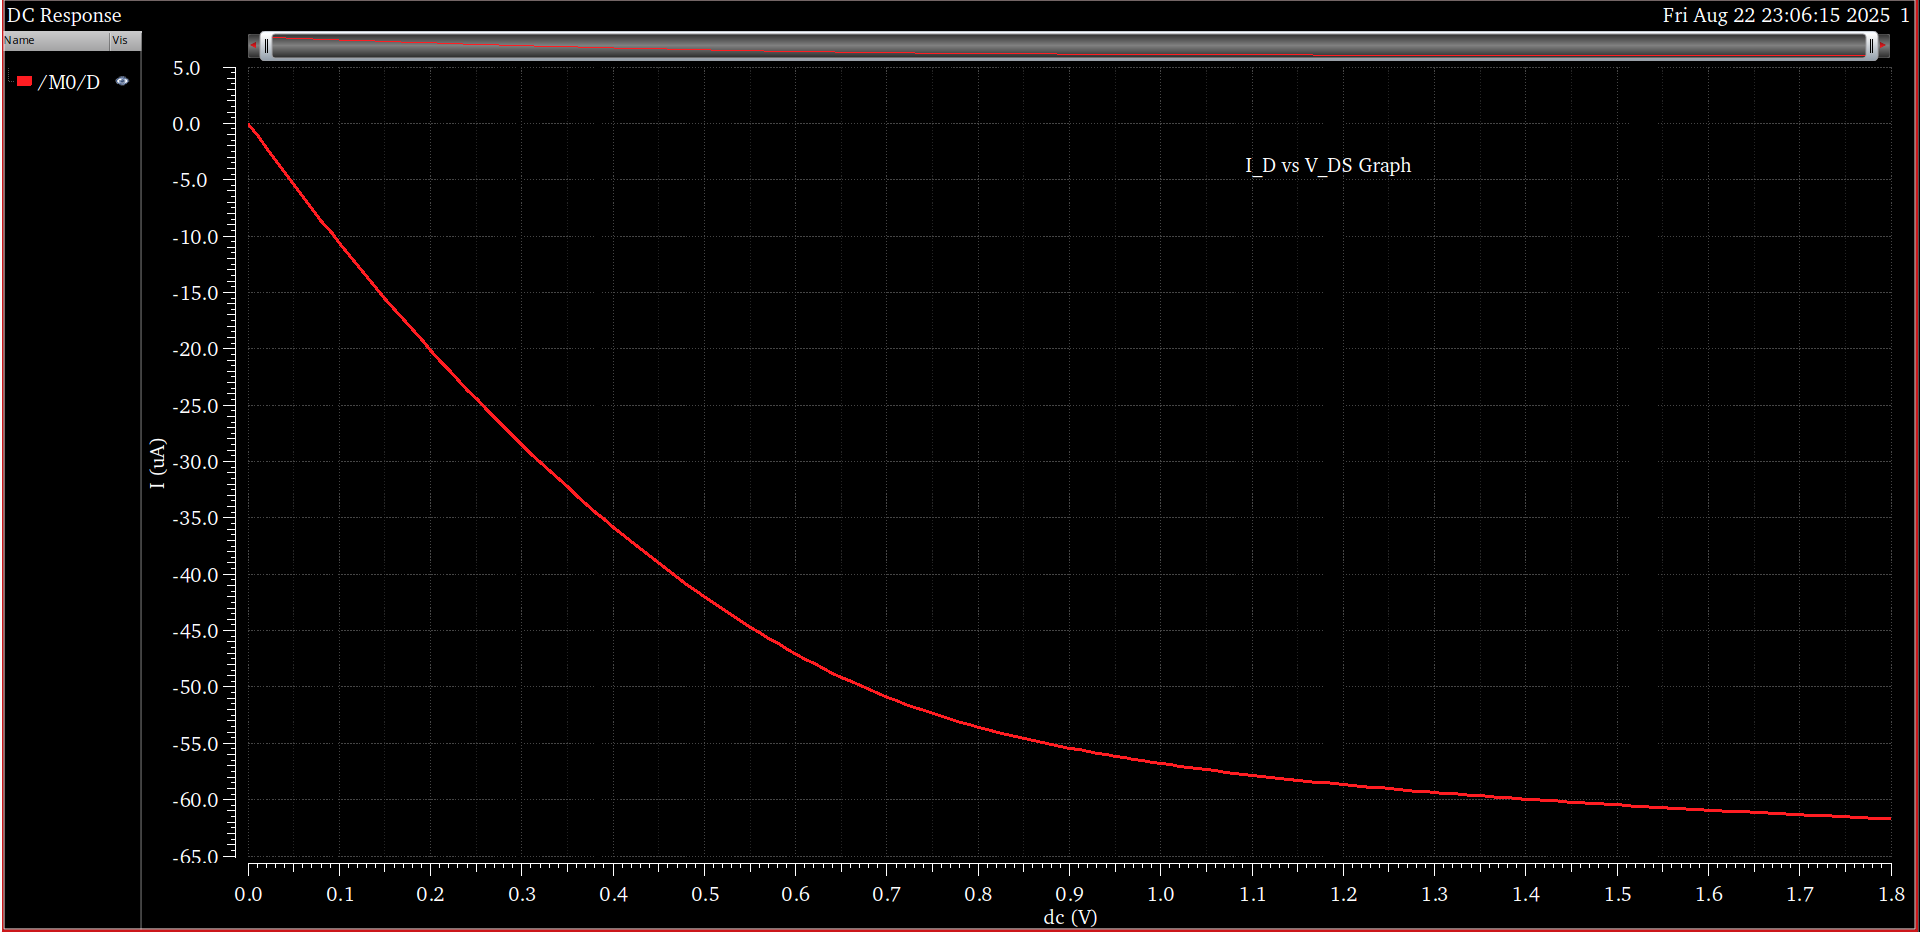
\includegraphics[width=0.8\textwidth]{images/pmos-I_D-vs-V_DS.png}
	\caption{$I_D$ vs $V_{DS}$ for PMOS}
	\label{fig:pmos-id-vs-vgs}
\end{figure}

\subsection{$I_D$ vs $V_{GS}$ for PMOS}
The following graph was obtained for $I_D$ vs $V_{GS}$ for the PMOS circuit from figure \ref{fig:pmos_circuit}:
\begin{figure}[h!]
	\centering
	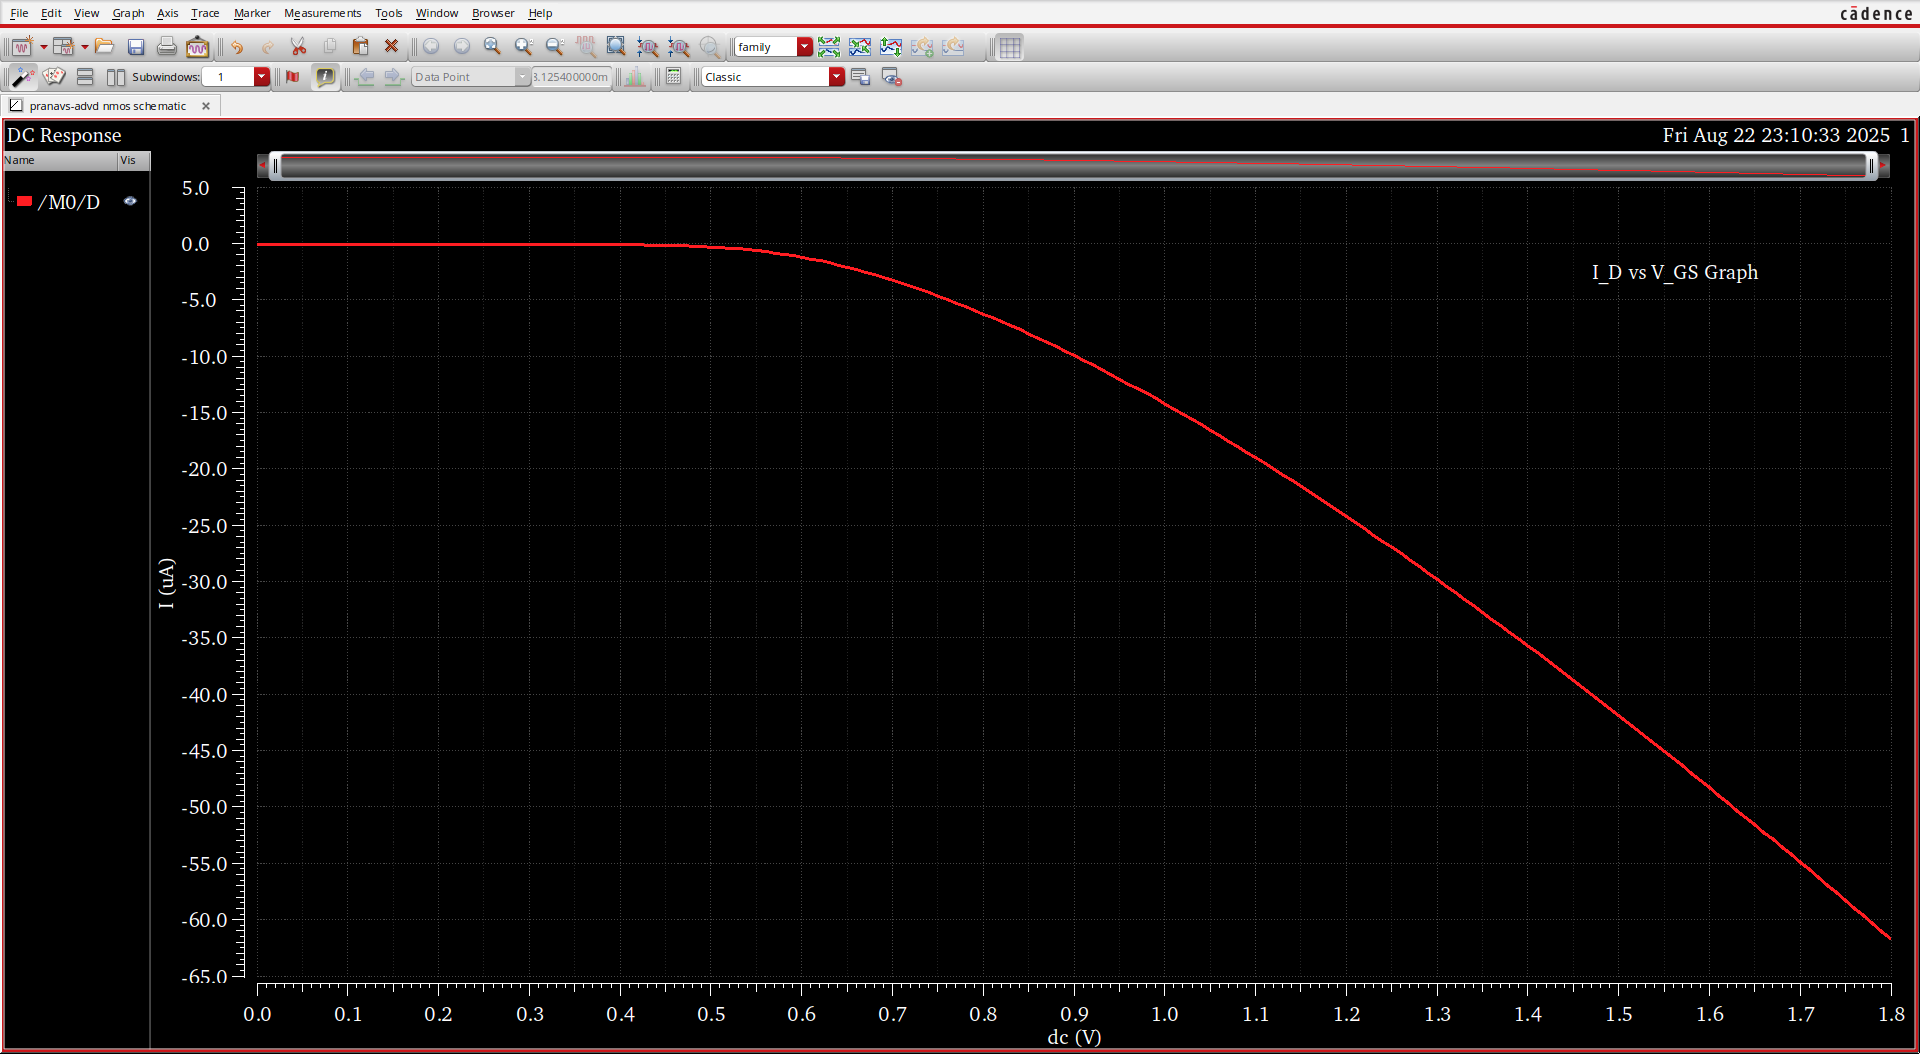
\includegraphics[width=0.8\textwidth]{images/pmos-I_D-vs-V_GS.png}
	\caption{$I_D$ vs $V_{GS}$ for PMOS}
	\label{fig:pmos-id-vs-vds}
\end{figure}

You can see the sharp cutoff at a certain voltage of $V_{GS}$, which indicates the threshold voltage $V_{th}$.

\end{document}
